% ─────────────────────────────────────────────────────────────────────────────
%  Seraph — Technical Reference Manual
%  Comprehensive backend + frontend documentation
% ─────────────────────────────────────────────────────────────────────────────
\documentclass[11pt,a4paper,twoside,openright]{book}

% ── Packages ─────────────────────────────────────────────────────────────────
\usepackage[T1]{fontenc}
\usepackage[utf8]{inputenc}
\usepackage{lmodern}
\usepackage{microtype}
\usepackage[top=25mm,bottom=25mm,inner=30mm,outer=25mm]{geometry}
\usepackage{graphicx}
\usepackage{xcolor}
\usepackage{booktabs}
\usepackage{longtable}
\usepackage{tabularx}
\usepackage{array}
\usepackage{listings}
\usepackage{fancyhdr}
\usepackage{titlesec}
\usepackage{tocloft}
\usepackage{hyperref}
\usepackage{enumitem}
\usepackage{mdframed}
\usepackage{fontawesome5}
\usepackage{amsmath}
\usepackage{float}
\usepackage{parskip}
\usepackage{multicol}
\usepackage{tikz}
\usepackage{pgfplots}
\pgfplotsset{compat=1.18}

% ── Colour palette ────────────────────────────────────────────────────────────
\definecolor{SeraphBg}{HTML}{0D0C0A}
\definecolor{SeraphAccent}{HTML}{F0A83A}
\definecolor{SeraphCrit}{HTML}{E85C4E}
\definecolor{SeraphHigh}{HTML}{E8783A}
\definecolor{SeraphMed}{HTML}{F0A83A}
\definecolor{SeraphLow}{HTML}{6B8A72}
\definecolor{SeraphFg}{HTML}{E8E0D0}
\definecolor{SeraphFg2}{HTML}{B8AFA0}
\definecolor{SeraphFg3}{HTML}{807870}
\definecolor{SeraphRule}{HTML}{2A2820}
\definecolor{SeraphCyan}{HTML}{5FB6C4}
\definecolor{SeraphViolet}{HTML}{B794F6}
\definecolor{codebg}{HTML}{1A1812}
\definecolor{codeframe}{HTML}{3A3828}

% ── Hyperref ─────────────────────────────────────────────────────────────────
\hypersetup{
  colorlinks = true,
  linkcolor  = SeraphAccent,
  urlcolor   = SeraphCyan,
  citecolor  = SeraphAccent,
  pdftitle   = {Seraph Technical Reference Manual},
  pdfauthor  = {Seraph Development Team},
  pdfsubject = {Cybersecurity Platform Documentation},
}

% ── Code listings ─────────────────────────────────────────────────────────────
\lstset{
  basicstyle      = \ttfamily\small,
  backgroundcolor = \color{codebg},
  frame           = single,
  rulecolor       = \color{codeframe},
  framesep        = 4pt,
  xleftmargin     = 8pt,
  xrightmargin    = 8pt,
  breaklines      = true,
  breakatwhitespace = true,
  postbreak       = \mbox{\textcolor{SeraphFg3}{$\hookrightarrow$}\space},
  showstringspaces = false,
  keywordstyle    = \color{SeraphAccent}\bfseries,
  commentstyle    = \color{SeraphFg3}\itshape,
  stringstyle     = \color{SeraphLow},
  numberstyle     = \tiny\color{SeraphFg3},
  numbers         = left,
  numbersep       = 8pt,
  tabsize         = 2,
}

\lstdefinelanguage{json}{
  morestring=[b]",
  literate=*
    {:}{{{\color{SeraphAccent}{:}}}}{1}
    {,}{{{\color{SeraphFg2}{,}}}}{1}
    {\{}{{{\color{SeraphCyan}{\{}}}}{1}
    {\}}{{{\color{SeraphCyan}{\}}}}}{1}
    {[}{{{\color{SeraphCyan}{[}}}}{1}
    {]}{{{\color{SeraphCyan}{]}}}}{1}
    {true}{{{\color{SeraphAccent}{true}}}}{4}
    {false}{{{\color{SeraphCrit}{false}}}}{5}
    {null}{{{\color{SeraphFg3}{null}}}}{4},
}

% ── Page style ────────────────────────────────────────────────────────────────
\pagestyle{fancy}
\fancyhf{}
\fancyhead[LE]{\small\color{SeraphFg3}\textsc{Seraph} \textbf{Technical Manual}}
\fancyhead[RO]{\small\color{SeraphFg3}\nouppercase{\leftmark}}
\fancyfoot[C]{\small\color{SeraphFg3}\thepage}
\renewcommand{\headrulewidth}{0.3pt}
\renewcommand{\headrule}{\hbox to\headwidth{\color{codeframe}\leaders\hrule height \headrulewidth\hfill}}

% ── Section formatting ────────────────────────────────────────────────────────
\titleformat{\chapter}[display]
  {\normalfont\huge\bfseries\color{SeraphAccent}}
  {\normalfont\Large\color{SeraphFg3}\MakeUppercase{\chaptertitlename}\ \thechapter}
  {12pt}{\Huge}
\titlespacing*{\chapter}{0pt}{-20pt}{30pt}

\titleformat{\section}
  {\normalfont\Large\bfseries\color{SeraphFg}}
  {\color{SeraphAccent}\thesection}{1em}{}
\titleformat{\subsection}
  {\normalfont\large\bfseries\color{SeraphFg}}
  {\color{SeraphFg3}\thesubsection}{1em}{}
\titleformat{\subsubsection}
  {\normalfont\normalsize\bfseries\color{SeraphFg2}}
  {\color{SeraphFg3}\thesubsubsection}{1em}{}

% ── Custom environments ───────────────────────────────────────────────────────
\newmdenv[
  backgroundcolor = codebg,
  linecolor       = codeframe,
  linewidth       = 1pt,
  leftmargin      = 0pt,
  rightmargin     = 0pt,
  innerleftmargin = 10pt,
  innerrightmargin= 10pt,
  innertopmargin  = 8pt,
  innerbottommargin=8pt,
]{codebox}

\newmdenv[
  backgroundcolor = SeraphBg,
  linecolor       = SeraphCrit,
  linewidth       = 2pt,
  topline         = false,
  bottomline      = false,
  rightline       = false,
  leftmargin      = 0pt,
  rightmargin     = 0pt,
  innerleftmargin = 12pt,
  innerrightmargin= 8pt,
  innertopmargin  = 6pt,
  innerbottommargin=6pt,
]{warningbox}

\newmdenv[
  backgroundcolor = SeraphBg,
  linecolor       = SeraphLow,
  linewidth       = 2pt,
  topline         = false,
  bottomline      = false,
  rightline       = false,
  leftmargin      = 0pt,
  rightmargin     = 0pt,
  innerleftmargin = 12pt,
  innerrightmargin= 8pt,
  innertopmargin  = 6pt,
  innerbottommargin=6pt,
]{notebox}

% ── Severity badge macro ──────────────────────────────────────────────────────
\newcommand{\sevbadge}[1]{%
  \ifstrequal{#1}{critical}{\colorbox{SeraphCrit}{\color{white}\tiny\textbf{CRITICAL}}}{}%
  \ifstrequal{#1}{high}{\colorbox{SeraphHigh}{\color{white}\tiny\textbf{HIGH}}}{}%
  \ifstrequal{#1}{medium}{\colorbox{SeraphMed}{\color{SeraphBg}\tiny\textbf{MEDIUM}}}{}%
  \ifstrequal{#1}{low}{\colorbox{SeraphLow}{\color{white}\tiny\textbf{LOW}}}{}%
}

% ── HTTP method macros ────────────────────────────────────────────────────────
\newcommand{\mget}{\colorbox{SeraphLow}{\color{white}\texttt{\footnotesize GET}}}
\newcommand{\mpost}{\colorbox{SeraphAccent}{\color{SeraphBg}\texttt{\footnotesize POST}}}
\newcommand{\mput}{\colorbox{SeraphCyan}{\color{SeraphBg}\texttt{\footnotesize PUT}}}
\newcommand{\mpatch}{\colorbox{SeraphViolet}{\color{SeraphBg}\texttt{\footnotesize PATCH}}}
\newcommand{\mdelete}{\colorbox{SeraphCrit}{\color{white}\texttt{\footnotesize DELETE}}}
\newcommand{\mws}{\colorbox{SeraphFg3}{\color{white}\texttt{\footnotesize WS}}}

% ── Table column helpers ──────────────────────────────────────────────────────
\newcolumntype{L}[1]{>{\raggedright\arraybackslash}p{#1}}
\newcolumntype{C}[1]{>{\centering\arraybackslash}p{#1}}

% ─────────────────────────────────────────────────────────────────────────────
\begin{document}

% ── Title page ────────────────────────────────────────────────────────────────
\begin{titlepage}
  \pagecolor{SeraphBg}
  \color{SeraphFg}
  \centering
  \vspace*{3cm}

  {\color{SeraphFg3}\footnotesize\textsc{confidential — internal reference}}
  \vspace{1.5cm}

  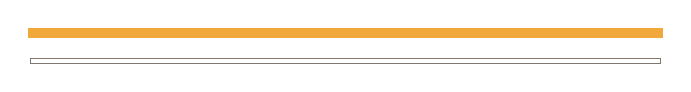
\begin{tikzpicture}
    \draw[color=SeraphAccent, line width=2pt] (0,0) rectangle (8,0.06);
    \draw[color=SeraphFg3,    line width=0.5pt] (0,-0.3) rectangle (8,-0.36);
  \end{tikzpicture}

  \vspace{1cm}
  {\color{SeraphAccent}\fontsize{64}{72}\selectfont\bfseries Seraph}

  \vspace{0.5cm}
  {\color{SeraphFg2}\Large Technical Reference Manual}

  \vspace{0.4cm}
  {\color{SeraphFg3}\normalsize Backend · Frontend · Architecture · API}

  \vspace{1.5cm}
  
\begin{tikzpicture}
    \draw[color=SeraphFg3, line width=0.5pt] (0,0) rectangle (8,-0.06);
  \end{tikzpicture}

  \vfill

  \begin{tabular}{@{}ll@{}}
    \color{SeraphFg3}\small Version & \color{SeraphFg}\small 0.1.0 \\[4pt]
    \color{SeraphFg3}\small Stack   & \color{SeraphFg}\small FastAPI · SQLAlchemy · React 18 · Electron \\[4pt]
    \color{SeraphFg3}\small Date    & \color{SeraphFg}\small \today \\
  \end{tabular}

  \vspace{2cm}
  
\begin{tikzpicture}
    \draw[color=SeraphAccent, line width=1pt] (0,0) rectangle (8,0.03);
  \end{tikzpicture}
  \vspace{0.5cm}
\end{titlepage}

\nopagecolor
\color{black}

% ── Front matter ──────────────────────────────────────────────────────────────
\frontmatter
\tableofcontents
\listoftables

% ─────────────────────────────────────────────────────────────────────────────
\mainmatter

% ═════════════════════════════════════════════════════════════════════════════
\chapter{Introduction \& Overview}
% ═════════════════════════════════════════════════════════════════════════════

\section{What is Seraph?}

Seraph is a \textbf{full-stack offensive security platform} designed for penetration testers and red team operators. It integrates reconnaissance, exploitation, post-exploitation, compliance auditing, credential management, and AI-assisted reporting into a single Electron desktop application backed by a FastAPI Python server.

\begin{notebox}
\textbf{Design philosophy.} Seraph is not a point tool — it is an \emph{engagement management layer} that orchestrates external security tools (Nmap, Metasploit, Nuclei, Hashcat, and 60+ others), stores all findings in a structured database, and presents them through a unified dark-themed interface.
\end{notebox}

\section{High-Level Architecture}

Seraph has three logical tiers:

\begin{enumerate}[leftmargin=*]
  \item \textbf{Desktop shell} (Electron 31) — Wraps the React renderer, exposes local Ollama LLM access via IPC, and persists window state.
  \item \textbf{Web frontend} (React 18 + Vite) — Single-page application served either from Electron or from FastAPI's static mount in server mode.
  \item \textbf{Backend API} (FastAPI + SQLAlchemy) — REST/WebSocket server handling all data, tool execution, and event streaming. Stores data in SQLite by default (PostgreSQL-ready).
\end{enumerate}

\begin{figure}[H]
\centering
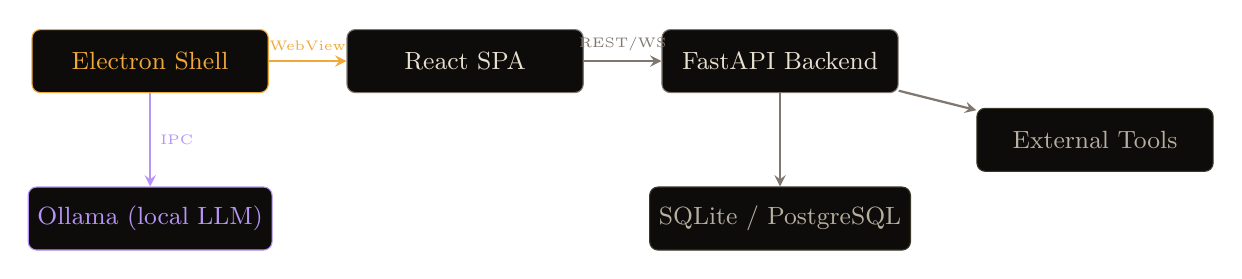
\begin{tikzpicture}[
  box/.style = {draw, rounded corners=3pt, minimum width=3cm, minimum height=0.8cm, align=center, font=\small},
  arr/.style = {->, >=stealth, thick}
]
  \node[box, fill=SeraphBg, text=SeraphAccent, draw=SeraphAccent] (electron) at (0,0) {Electron Shell};
  \node[box, fill=SeraphBg, text=SeraphFg,    draw=SeraphFg3]    (react)    at (4,0) {React SPA};
  \node[box, fill=SeraphBg, text=SeraphFg,    draw=SeraphFg3]    (fastapi)  at (8,0) {FastAPI Backend};
  \node[box, fill=SeraphBg, text=SeraphFg2,   draw=codeframe]    (sqlite)   at (8,-2) {SQLite / PostgreSQL};
  \node[box, fill=SeraphBg, text=SeraphFg2,   draw=codeframe]    (tools)    at (12,-1) {External Tools};
  \node[box, fill=SeraphBg, text=SeraphViolet, draw=SeraphViolet] (ollama)   at (0,-2) {Ollama (local LLM)};

  \draw[arr, color=SeraphAccent] (electron) -- (react) node[midway, above, font=\tiny] {WebView};
  \draw[arr, color=SeraphFg3]    (react)    -- (fastapi) node[midway, above, font=\tiny] {REST/WS};
  \draw[arr, color=SeraphFg3]    (fastapi)  -- (sqlite);
  \draw[arr, color=SeraphFg3]    (fastapi)  -- (tools);
  \draw[arr, color=SeraphViolet] (electron) -- (ollama) node[midway, right, font=\tiny] {IPC};
\end{tikzpicture}
\caption{Seraph system architecture}
\end{figure}

\section{Core Capabilities}

\begin{multicols}{2}
\begin{itemize}[leftmargin=*,noitemsep]
  \item Project-scoped engagement management
  \item Multi-target asset tracking
  \item Automated tool orchestration (60+ tools)
  \item Metasploit C2 session management
  \item Post-exploitation automation (playbooks)
  \item Remote agent deployment
  \item Compliance auditing (CIS, NIST, STIG)
  \item Hash cracking (Hashcat, John)
  \item OSINT reconnaissance pipeline
  \item CVE monitoring and alerting
  \item Encrypted credential vault (AES-256-GCM)
  \item AI-assisted triage and reporting (Ollama)
  \item Event-driven listeners and webhooks
  \item Real-time streaming via WebSockets
  \item PDF/HTML/Markdown report generation
\end{itemize}
\end{multicols}

% ═════════════════════════════════════════════════════════════════════════════
\chapter{Backend}
% ═════════════════════════════════════════════════════════════════════════════

\section{Technology Stack}

\begin{table}[H]
\centering
\begin{tabularx}{\textwidth}{L{3cm} L{3.5cm} X}
\toprule
\textbf{Layer} & \textbf{Technology} & \textbf{Role} \\
\midrule
Web framework   & FastAPI (async)         & HTTP/WebSocket API, middleware, lifespan hooks \\
ORM             & SQLAlchemy 2.0          & Async models, migrations (Alembic) \\
Database        & SQLite (default)        & File-based storage; PostgreSQL supported via URL env var \\
Auth            & PyJWT + bcrypt          & JWT access tokens + API token hashing \\
Scheduling      & APScheduler             & Cron-based automated scans \\
MSF RPC         & pymetasploit3           & Metasploit Framework integration \\
Templating      & Jinja2                  & HTML/Markdown report rendering \\
AI/LLM          & httpx (Ollama REST)     & Narrative generation, remediation, log triage \\
\bottomrule
\end{tabularx}
\caption{Backend technology stack}
\end{table}

\section{File Structure}

\begin{codebox}
\begin{lstlisting}[language=bash, numbers=none]
seraph/
├── backend/
│   ├── main.py              # FastAPI app factory, middleware, routers
│   ├── config.py            # Pydantic BaseSettings (env vars)
│   ├── database.py          # SQLAlchemy models + create_tables()
│   ├── dependencies.py      # get_current_user(), DB session
│   ├── vault.py             # AES-256-GCM encryption helpers
│   ├── routers/             # 24 API modules (one per domain)
│   │   ├── auth.py          # JWT, users, API tokens, passkeys
│   │   ├── projects.py      # Projects, targets, stats
│   │   ├── audit.py         # CIS/NIST audit builder
│   │   ├── pentest.py       # Pentest workbench tool execution
│   │   ├── c2.py            # C2/MSF session management (66 KB)
│   │   ├── credentials.py   # Encrypted credential vault
│   │   ├── vulns.py         # Vulnerability tracker + AI remediation
│   │   ├── cve_watch.py     # CVE feed monitoring
│   │   ├── playbooks.py     # Automation workflows
│   │   ├── agents.py        # Remote agent management
│   │   ├── ai.py            # LLM config + narrative/chat
│   │   ├── logs.py          # Log analysis + AI triage
│   │   ├── osint.py         # OSINT module runner
│   │   ├── network.py       # Network topology
│   │   ├── enrichment.py    # NVD/CVE enrichment
│   │   ├── hardening.py     # Hardening reports
│   │   ├── profiles.py      # Scan profiles
│   │   ├── listeners.py     # Event-driven monitors
│   │   ├── notifications.py # In-app notifications
│   │   ├── webhooks.py      # Outbound webhooks
│   │   ├── cracking.py      # Hash cracking jobs
│   │   ├── demo.py          # Demo data seed/clear
│   │   ├── settings.py      # App settings API
│   │   └── ws.py            # All WebSocket endpoints
│   ├── services/
│   │   ├── tool_registry.py # Tool detection + metadata (60+ tools)
│   │   ├── msf_client.py    # Metasploit RPC wrapper
│   │   ├── scheduler.py     # APScheduler + cron execution
│   │   ├── playbook_runner.py # Async playbook execution engine
│   │   ├── listener_manager.py # Event listener polling
│   │   ├── cve_watcher.py   # CVE feed polling
│   │   └── auth_service.py  # Login, token, brute-force tracking
│   ├── data/
│   │   └── tool_chains.json # Tool chain definitions
│   ├── templates/           # Jinja2 report templates
│   └── alembic/             # Schema migration scripts
└── .env.example
\end{lstlisting}
\end{codebox}

\section{Startup Sequence}

On process start FastAPI's \texttt{lifespan} hook runs the following steps in order:

\begin{enumerate}[leftmargin=*]
  \item \textbf{\texttt{create\_tables()}} --- SQLAlchemy \texttt{Base.metadata.create\_all()} creates any missing tables without dropping existing data.
  \item \textbf{\texttt{\_reset\_stale\_scans()}} --- Any scan with \texttt{status = running} is set to \texttt{failed}. This prevents zombie entries after a hard restart.
  \item \textbf{\texttt{initialize\_registry()}} --- Detects all available CLI security tools using \texttt{shutil.which()} across standard and extra paths (\texttt{\~/go/bin}, \texttt{\~/.cargo/bin}, \texttt{/snap/bin}, etc.).
  \item \textbf{\texttt{initialize\_scheduler()}} --- Starts APScheduler and schedules any \texttt{ScanProfile} rows with non-null \texttt{schedule} cron expressions.
  \item \textbf{\texttt{initialize\_listeners()}} --- Activates event listener background polling.
  \item \textbf{\texttt{seed\_builtin\_playbooks()}} --- Inserts built-in playbook definitions if not already present (idempotent upsert).
\end{enumerate}

\section{Middleware Stack}

\begin{table}[H]
\centering
\begin{tabularx}{\textwidth}{L{3.5cm} X}
\toprule
\textbf{Middleware} & \textbf{Behaviour} \\
\midrule
CORS & Configurable allowed origins; Electron's \texttt{null} origin supported via \texttt{SERAPH\_EXTRA\_CORS\_ORIGINS}. Regex fallback for LAN testing. \\
Rate Limiting & Default 300 requests/60 s per IP. Authenticated users get a 5× burst multiplier. WebSocket (\texttt{/ws/*}) and static (\texttt{/assets/*}) paths are exempt. \\
Audit Logging & All \texttt{POST}, \texttt{PUT}, \texttt{PATCH}, \texttt{DELETE} requests to \texttt{/api/v1/*} are written to \texttt{AuditLog} with actor user ID, IP, resource type, and resource ID. \\
\bottomrule
\end{tabularx}
\caption{Backend middleware stack}
\end{table}

\section{Configuration \& Environment Variables}

\begin{table}[H]
\centering
\begin{tabularx}{\textwidth}{L{5.5cm} L{4cm} X}
\toprule
\textbf{Variable} & \textbf{Default} & \textbf{Description} \\
\midrule
\texttt{SERAPH\_DATABASE\_URL}    & \texttt{sqlite:///./seraph.db} & SQLAlchemy connection URL \\
\texttt{SERAPH\_SECRET\_KEY}      & random per process & JWT signing secret (set in production) \\
\texttt{SERAPH\_RP\_ID}           & \texttt{localhost}             & WebAuthn relying party ID \\
\texttt{SERAPH\_RP\_ORIGINS}      & localhost variants             & Comma-separated allowed WebAuthn origins \\
\texttt{SERAPH\_EXTRA\_CORS\_ORIGINS} & (empty)                    & Additional CORS origins; use \texttt{null} for Electron \\
\texttt{SERAPH\_RATE\_LIMIT\_WINDOW}  & \texttt{60}                & Rate limit window in seconds \\
\texttt{SERAPH\_RATE\_LIMIT\_REQUESTS}& \texttt{300}               & Max requests per window per IP \\
\texttt{SERAPH\_RATE\_LIMIT\_BURST}   & \texttt{5}                 & Multiplier for authenticated users \\
\texttt{MSF\_RPC\_PASSWORD}       & (required for C2)              & Metasploit RPC daemon password \\
\bottomrule
\end{tabularx}
\caption{Environment variables}
\end{table}

Runtime settings (AI config, auto post-exploitation) are stored in the \texttt{AppSetting} table as key/value rows and are readable/writable via \texttt{GET/PUT /api/v1/settings}.

\section{Authentication \& Authorisation}

\subsection{JWT Flow}

\begin{enumerate}[leftmargin=*]
  \item Client posts credentials to \texttt{POST /api/v1/auth/login}.
  \item Server validates bcrypt hash, checks IP lockout (5 failed attempts → 5-minute block).
  \item Returns an access token (24-hour expiry, signed with \texttt{SERAPH\_SECRET\_KEY}).
  \item Token payload contains: \texttt{sub} (user UUID), \texttt{jti} (token ID for revocation), \texttt{role}, \texttt{exp}.
  \item All protected routes use the \texttt{get\_current\_user} FastAPI dependency which validates the JWT and cross-checks \texttt{jti} against the \texttt{RevokedToken} table.
\end{enumerate}

\subsection{API Tokens}

Long-lived tokens (format: \texttt{srph\_<32 random chars>}) are issued for programmatic access by Chronos, remote agents, and CI pipelines. Only the SHA-256 hash plus the first 8-character prefix are stored — the full token is shown once at creation time.

\subsection{WebAuthn / Passkeys}

Browser-based passkey authentication is supported for operator desktops. The relying party ID and allowed origins are configurable. The \texttt{PasskeyCredential} table stores COSE public keys and sign-count for replay protection.

\section{Database Schema}

\subsection{Core Entities}

\begin{table}[H]
\centering
\begin{tabularx}{\textwidth}{L{3cm} L{4cm} X}
\toprule
\textbf{Model} & \textbf{Key Fields} & \textbf{Notes} \\
\midrule
\texttt{Project}   & id (UUID), name, description, scope\_json, created\_at & Root engagement container. Cascade-deletes targets, scans, findings. \\
\texttt{Target}    & hostname\_or\_ip, target\_type, ports, notes & Types: \texttt{linux\_host}, \texttt{windows\_host}, \texttt{web\_app}, \texttt{cloud\_*}, \texttt{network}, \texttt{api\_endpoint}. \\
\texttt{Scan}      & scan\_type, module, status, config\_json, raw\_output, started\_at, completed\_at & Statuses: \texttt{pending}, \texttt{running}, \texttt{completed}, \texttt{failed}. \\
\texttt{Finding}   & severity, title, description, cve\_id, cvss\_score, status, tags, exploit\_chain\_json & Severity enum: \texttt{critical}, \texttt{high}, \texttt{medium}, \texttt{low}. Status: \texttt{open}, \texttt{in-review}, \texttt{remediated}, \texttt{accepted}. \\
\bottomrule
\end{tabularx}
\caption{Core entity models (cascade chain: Project → Target → Scan → Finding)}
\end{table}

\subsection{C2 \& Post-Exploitation Models}

\begin{table}[H]
\centering
\begin{tabularx}{\textwidth}{L{3cm} L{4.5cm} X}
\toprule
\textbf{Model} & \textbf{Key Fields} & \textbf{Notes} \\
\midrule
\texttt{C2Session}  & msf\_session\_id, session\_type, platform, arch, remote\_host, remote\_port, tunnel\_peer, via\_exploit, via\_payload, status, checklist\_json, sysinfo\_json, pivot\_routes\_json & Status: \texttt{active}, \texttt{inactive}, \texttt{lost}. \\
\texttt{LootEntry}  & loot\_type, title, content, source\_path, captured\_at & Types: credential, hash, file, etc. \\
\texttt{C2Task}     & command, output, status, executed\_at, completed\_at & Status: \texttt{pending}, \texttt{running}, \texttt{done}, \texttt{error}. \\
\bottomrule
\end{tabularx}
\caption{C2 and post-exploitation models}
\end{table}

\subsection{Security \& Vault Models}

\begin{table}[H]
\centering
\begin{tabularx}{\textwidth}{L{3cm} L{4.5cm} X}
\toprule
\textbf{Model} & \textbf{Key Fields} & \textbf{Notes} \\
\midrule
\texttt{Credential}         & project\_id, username, secret\textsuperscript{enc}, cred\_type, source, target\_host, notes\textsuperscript{enc} & \texttt{secret} and \texttt{notes} stored as AES-256-GCM ciphertext via custom SQLAlchemy type. \\
\texttt{VulnerabilityRecord}& project\_id, title, severity, status, cvss\_score, cve\_id, affected\_asset, ai\_remediation, tags & Tracks remediable issues separate from raw scan findings. \\
\texttt{WatchedService}     & target\_id, service\_term, last\_checked, known\_cves & Polled against CVE feeds on schedule. \\
\texttt{FPSuppressionRule}  & project\_id, tool, title\_contains & False positive filters applied during scan parsing. \\
\bottomrule
\end{tabularx}
\caption{Security and vault models}
\end{table}

\subsection{Automation Models}

\begin{table}[H]
\centering
\begin{tabularx}{\textwidth}{L{3cm} L{4.5cm} X}
\toprule
\textbf{Model} & \textbf{Key Fields} & \textbf{Notes} \\
\midrule
\texttt{Playbook}    & name, description, steps\_json, is\_builtin & Steps serialised as JSON array with parallel flag support. \\
\texttt{PlaybookRun} & playbook\_id, project\_id, target\_id, mode, status, current\_step, results\_json & Mode: \texttt{auto} or \texttt{step\_through}. \\
\texttt{ScanProfile} & name, scan\_categories, schedule, scheduled\_project\_id, last\_run, next\_run & Cron expr drives APScheduler. \\
\texttt{Agent}       & name, target\_id, token, short\_code, hostname, platform, status, last\_seen & Status: \texttt{online} / \texttt{offline}. \\
\texttt{AgentJob}    & agent\_id, scan\_id, categories, script, status, output, exit\_code & Long-polled by agent; result posted back. \\
\texttt{Listener}    & name, type, project\_id, target\_id, config\_json, status & Types: \texttt{scheduled}, \texttt{threshold}, \texttt{healthcheck}. \\
\texttt{Notification}& title, body, type, read, scan\_id & Types: \texttt{info}, \texttt{warning}, \texttt{critical}. Broadcast via \texttt{/ws/events}. \\
\bottomrule
\end{tabularx}
\caption{Automation and monitoring models}
\end{table}

\subsection{Auth \& Audit Models}

\begin{table}[H]
\centering
\begin{tabularx}{\textwidth}{L{3.5cm} L{4cm} X}
\toprule
\textbf{Model} & \textbf{Key Fields} & \textbf{Notes} \\
\midrule
\texttt{User}              & username, hashed\_password, role, full\_name & Roles: \texttt{admin}, \texttt{analyst}. \\
\texttt{ApiToken}          & user\_id, name, token\_hash, prefix, last\_used\_at & SHA-256 hash only stored. \\
\texttt{RevokedToken}      & jti, revoked\_at, expires\_at & Checked on every authenticated request. \\
\texttt{PasskeyCredential} & user\_id, credential\_id, public\_key, sign\_count, name & COSE public key; WebAuthn spec. \\
\texttt{AuditLog}          & action, user\_id, resource\_type, resource\_id, ip\_address, created\_at & Written by audit middleware for all mutations. \\
\texttt{AppSetting}        & key (PK), value & Flexible config store (AI params, auto-probe flags). \\
\bottomrule
\end{tabularx}
\caption{Auth and audit models}
\end{table}

\section{API Reference}

All endpoints are prefixed \texttt{/api/v1}. Protected endpoints require \texttt{Authorization: Bearer <token>}.

\subsection{Authentication}

\begin{longtable}{L{1.2cm} L{5.5cm} X}
\toprule
\textbf{Method} & \textbf{Path} & \textbf{Description} \\
\midrule
\endhead
\mget    & \texttt{/auth/setup-required}        & Returns \texttt{\{required: bool\}} — true if no users exist yet. \\
\mpost   & \texttt{/auth/setup}                 & Creates the first admin user (201). Disabled after first call. \\
\mpost   & \texttt{/auth/login}                 & Returns JWT access token. Subject to IP-based rate limiting. \\
\mpost   & \texttt{/auth/logout}                & Revokes the current token (adds JTI to \texttt{RevokedToken}). \\
\mget    & \texttt{/auth/me}                    & Returns current user object with role. \\
\mpatch  & \texttt{/auth/me}                    & Update own \texttt{full\_name}. \\
\mpost   & \texttt{/auth/change-password}       & Change own password; validates current password first. \\
\mpost   & \texttt{/auth/users}                 & Admin: create a new user. \\
\mget    & \texttt{/auth/users}                 & Admin: list all users. \\
\mdelete & \texttt{/auth/users/\{user\_id\}}    & Admin: delete a user. \\
\mpost   & \texttt{/auth/tokens}                & Generate a long-lived API token. \\
\mget    & \texttt{/auth/tokens}                & List own API tokens (shows prefix only). \\
\mdelete & \texttt{/auth/tokens/\{token\_id\}}  & Revoke an API token. \\
\bottomrule
\caption{Authentication endpoints}
\end{longtable}

\subsection{Projects \& Targets}

\begin{longtable}{L{1.2cm} L{5.5cm} X}
\toprule
\textbf{Method} & \textbf{Path} & \textbf{Description} \\
\midrule
\endhead
\mget    & \texttt{/projects}                        & List all projects with finding counts per severity. \\
\mpost   & \texttt{/projects}                        & Create a new project (name, description). \\
\mget    & \texttt{/projects/\{id\}}                 & Project detail including targets. \\
\mput    & \texttt{/projects/\{id\}}                 & Update name or description. \\
\mdelete & \texttt{/projects/\{id\}}                 & Delete project and all child entities. \\
\mget    & \texttt{/projects/\{id\}/targets}         & List targets for a project. \\
\mpost   & \texttt{/projects/\{id\}/targets}         & Add a target (hostname\_or\_ip, target\_type, ports, notes). \\
\mput    & \texttt{/projects/\{id\}/scope}           & Update include/exclude CIDR blocks. \\
\mget    & \texttt{/targets/\{id\}}                  & Single target detail. \\
\mput    & \texttt{/targets/\{id\}}                  & Update target fields. \\
\mdelete & \texttt{/targets/\{id\}}                  & Delete target (cascades to scans). \\
\mget    & \texttt{/stats}                           & Platform-wide KPIs: project count, scan totals, finding severities. \\
\mget    & \texttt{/findings}                        & Cross-project findings (filterable by \texttt{project\_id}, \texttt{severity}, \texttt{status}). \\
\bottomrule
\caption{Project and target endpoints}
\end{longtable}

\subsection{Audit Builder}

The Audit Builder generates bash scripts from compliance benchmark control selections, executes them against targets, and parses results into findings.

\begin{longtable}{L{1.2cm} L{6.5cm} X}
\toprule
\textbf{Method} & \textbf{Path} & \textbf{Description} \\
\midrule
\endhead
\mget    & \texttt{/audit/categories}                      & Available audit scan categories (CIS L1/L2, NIST, Lynis, etc.). \\
\mpost   & \texttt{/audit/generate}                        & Generate a bash audit script for selected categories and target. \\
\mget    & \texttt{/audit/script/\{scan\_id\}/download}    & Download the generated script. \\
\mpost   & \texttt{/audit/scans}                           & Create an audit scan from uploaded output JSON. \\
\mget    & \texttt{/audit/scans}                           & List audit scans (filterable by project). \\
\mget    & \texttt{/audit/scans/\{scan\_id\}}              & Scan detail with associated findings. \\
\mpost   & \texttt{/audit/scans/\{scan\_id\}/parse}        & Re-parse raw scan output to (re-)generate findings. \\
\mget    & \texttt{/audit/findings}                        & Findings from audit scans (filterable by project). \\
\mpost   & \texttt{/audit/reports/generate}                & Generate a formatted report (HTML/Markdown). \\
\mget    & \texttt{/audit/reports/download/\{project\_id\}} & Download the latest report for a project. \\
\mpost   & \texttt{/audit/import}                          & Import audit results from a JSON/JSONL file. \\
\bottomrule
\caption{Audit Builder endpoints}
\end{longtable}

\subsection{Pentest Workbench}

\begin{longtable}{L{1.2cm} L{6.5cm} X}
\toprule
\textbf{Method} & \textbf{Path} & \textbf{Description} \\
\midrule
\endhead
\mget    & \texttt{/pentest/engagements}                     & List engagement phases (recon, scanning, exploitation, \ldots). \\
\mget    & \texttt{/pentest/engagements/\{type\}/phases/\{id\}} & Tools available for a specific phase. \\
\mpost   & \texttt{/pentest/run}                             & Execute a pentest tool; creates a \texttt{Scan} record and streams output via WebSocket. \\
\mget    & \texttt{/pentest/scans}                           & List pentest scans. \\
\mget    & \texttt{/pentest/scans/\{scan\_id\}}              & Single scan with raw output and parsed findings. \\
\bottomrule
\caption{Pentest workbench endpoints}
\end{longtable}

\subsection{C2 / Post-Exploitation}

The C2 router (\texttt{c2.py}, 66 KB) is the largest in the codebase, reflecting the depth of Metasploit integration.

\begin{longtable}{L{1.2cm} L{6.5cm} X}
\toprule
\textbf{Method} & \textbf{Path} & \textbf{Description} \\
\midrule
\endhead
\multicolumn{3}{l}{\textit{Connection}} \\
\mpost   & \texttt{/c2/connect}                   & Connect to Metasploit RPC daemon. \\
\mpost   & \texttt{/c2/disconnect}                & Disconnect from MSF RPC. \\
\mget    & \texttt{/c2/status}                    & MSF status: version, sessions, active jobs. \\
\midrule
\multicolumn{3}{l}{\textit{Sessions}} \\
\mget    & \texttt{/c2/sessions}                  & List all C2 sessions. \\
\mpost   & \texttt{/c2/sessions/sync}             & Sync sessions from live MSF. \\
\mpost   & \texttt{/c2/sessions}                  & Register a session manually. \\
\mpatch  & \texttt{/c2/sessions/\{id\}/status}    & Update session status (active/inactive/lost). \\
\mdelete & \texttt{/c2/sessions/\{id\}}           & Remove a session record. \\
\mpost   & \texttt{/c2/sessions/\{id\}/exec}      & Execute a command on the session. \\
\mget    & \texttt{/c2/sessions/\{id\}/tasks}     & History of commands executed in the session. \\
\mpost   & \texttt{/c2/sessions/\{id\}/sysinfo}   & Run system enumeration commands. \\
\mget    & \texttt{/c2/sessions/\{id\}/sysinfo}   & Retrieve gathered system info. \\
\midrule
\multicolumn{3}{l}{\textit{Post-Exploitation}} \\
\mget    & \texttt{/c2/post-modules}              & List available post-exploitation modules. \\
\mpost   & \texttt{/c2/post-modules/run}          & Execute a post module on a session. \\
\mget    & \texttt{/c2/sessions/\{id\}/checklist} & Post-ex checklist state. \\
\mpatch  & \texttt{/c2/sessions/\{id\}/checklist/\{item\_id\}} & Mark a checklist item complete. \\
\mpost   & \texttt{/c2/sessions/\{id\}/auto-probe}& Run auto-probe (system enumeration + auto checklist). \\
\mpost   & \texttt{/c2/sessions/\{id\}/upgrade}   & Attempt privilege escalation. \\
\mpost   & \texttt{/c2/sessions/\{id\}/lateral-discover} & Identify pivot targets. \\
\mget    & \texttt{/c2/sessions/\{id\}/routes}    & Pivot routes through this session. \\
\mpost   & \texttt{/c2/sessions/\{id\}/routes}    & Add a pivot route. \\
\mdelete & \texttt{/c2/sessions/\{id\}/routes/\{id\}} & Remove a route. \\
\midrule
\multicolumn{3}{l}{\textit{Loot}} \\
\mget    & \texttt{/c2/loot}                      & All loot across sessions. \\
\mpost   & \texttt{/c2/loot}                      & Add loot entry (credential, hash, file, etc.). \\
\mpost   & \texttt{/c2/loot/sync-msf}             & Pull loot from MSF loot database. \\
\mdelete & \texttt{/c2/loot/\{id\}}               & Delete a loot entry. \\
\midrule
\multicolumn{3}{l}{\textit{Payloads \& Listeners}} \\
\mget    & \texttt{/c2/payloads}                  & List available payload types (meterpreter, shell, etc.). \\
\mpost   & \texttt{/c2/payloads/generate}         & Generate a payload binary/script. \\
\mpost   & \texttt{/c2/listeners/start}           & Start a Metasploit handler/listener. \\
\mget    & \texttt{/c2/listeners}                 & List active listeners. \\
\mdelete & \texttt{/c2/listeners/\{id\}}          & Stop a listener. \\
\midrule
\multicolumn{3}{l}{\textit{Utilities}} \\
\mpost   & \texttt{/c2/attack-plan}               & Map CVEs to recommended MSF modules. \\
\mget    & \texttt{/c2/lotl}                      & Living-off-the-land binaries reference database. \\
\bottomrule
\caption{C2 and post-exploitation endpoints}
\end{longtable}

\subsection{Credentials, Findings \& Vulnerabilities}

\begin{longtable}{L{1.2cm} L{6cm} X}
\toprule
\textbf{Method} & \textbf{Path} & \textbf{Description} \\
\midrule
\endhead
\mget    & \texttt{/credentials}              & List all credentials in the vault. \\
\mpost   & \texttt{/credentials}              & Add a credential (secret encrypted AES-256-GCM at rest). \\
\mget    & \texttt{/credentials/\{id\}}       & Retrieve a single credential (secret decrypted). \\
\mdelete & \texttt{/credentials/\{id\}}       & Delete a credential. \\
\mget    & \texttt{/vulns}                    & List vulnerability records across projects. \\
\mput    & \texttt{/vulns/\{id\}}             & Update vuln status, remediation notes. \\
\mpost   & \texttt{/vulns/\{id\}/ai-remediate}& Generate AI-assisted remediation steps via local LLM. \\
\mget    & \texttt{/findings/\{id\}/notes}    & Notes/comments on a finding. \\
\mpost   & \texttt{/findings/\{id\}/notes}    & Add a note to a finding. \\
\mdelete & \texttt{/findings/notes/\{id\}}    & Delete a note. \\
\mdelete & \texttt{/findings/\{id\}}          & Delete a finding. \\
\bottomrule
\caption{Credentials, findings, and vulnerability endpoints}
\end{longtable}

\subsection{CVE Watch, AI, and Other Endpoints}

\begin{longtable}{L{1.2cm} L{6.5cm} X}
\toprule
\textbf{Method} & \textbf{Path} & \textbf{Description} \\
\midrule
\endhead
\multicolumn{3}{l}{\textit{CVE Watch}} \\
\mget    & \texttt{/cve-watch}             & List watched services. \\
\mpost   & \texttt{/cve-watch}             & Add a service to watch. \\
\mdelete & \texttt{/cve-watch/\{id\}}      & Stop watching a service. \\
\mpost   & \texttt{/cve-watch/\{id\}/check}& Check a single service for new CVEs now. \\
\mpost   & \texttt{/cve-watch/check-all}   & Check all watched services. \\
\midrule
\multicolumn{3}{l}{\textit{AI / LLM}} \\
\mget    & \texttt{/ai/config}             & Get current LLM endpoint config. \\
\mput    & \texttt{/ai/config}             & Update LLM endpoint (Ollama, LMStudio). \\
\mget    & \texttt{/ai/status}             & Test LLM connectivity. \\
\mget    & \texttt{/ai/models}             & List models available at the configured endpoint. \\
\mpost   & \texttt{/ai/narrate}            & Generate AI narrative for a project's findings. \\
\mpost   & \texttt{/ai/chat}               & Chat completion for the AI Operator. \\
\midrule
\multicolumn{3}{l}{\textit{Notifications}} \\
\mget    & \texttt{/notifications}         & List all notifications for current user. \\
\mpatch  & \texttt{/notifications/\{id\}/read} & Mark a notification read. \\
\mpatch  & \texttt{/notifications/read-all}& Mark all notifications read. \\
\mdelete & \texttt{/notifications/read}    & Clear all read notifications. \\
\midrule
\multicolumn{3}{l}{\textit{Playbooks}} \\
\mget    & \texttt{/playbooks}             & List built-in and custom playbooks. \\
\mpost   & \texttt{/playbooks}             & Create a custom playbook. \\
\mget    & \texttt{/playbooks/\{id\}}      & Get playbook with steps. \\
\mdelete & \texttt{/playbooks/\{id\}}      & Delete a custom playbook. \\
\mpost   & \texttt{/playbooks/\{id\}/run}  & Execute a playbook on a project/target. \\
\midrule
\multicolumn{3}{l}{\textit{Agents}} \\
\mpost   & \texttt{/agents}                    & Register a new agent. \\
\mget    & \texttt{/agents}                    & List agents with online/offline status. \\
\mdelete & \texttt{/agents/\{id\}}             & Remove an agent. \\
\mget    & \texttt{/agents/\{id\}/install-script}& Shell script to install the agent binary. \\
\mpost   & \texttt{/agents/\{id\}/jobs}        & Queue a job on an agent. \\
\mget    & \texttt{/poll/\{token\}}            & Long-poll endpoint (agent retrieves queued jobs). \\
\mpost   & \texttt{/result/\{token\}/\{job\_id\}}& Agent submits job result. \\
\midrule
\multicolumn{3}{l}{\textit{Webhooks}} \\
\mget    & \texttt{/webhooks}              & List webhook configs. \\
\mpost   & \texttt{/webhooks}              & Create a webhook (URL, event types, optional HMAC secret). \\
\mdelete & \texttt{/webhooks/\{id\}}       & Delete a webhook. \\
\bottomrule
\caption{CVE watch, AI, notifications, playbooks, agents, and webhook endpoints}
\end{longtable}

\subsection{WebSocket Endpoints}

\begin{table}[H]
\centering
\begin{tabularx}{\textwidth}{L{5.5cm} X}
\toprule
\textbf{Path} & \textbf{Purpose} \\
\midrule
\texttt{/ws/execute/\{scan\_id\}}      & Stream tool output line-by-line during scan execution. \\
\texttt{/ws/pentest/\{scan\_id\}}      & Stream pentest tool execution (Nmap, Nuclei, etc.). \\
\texttt{/ws/osint/\{scan\_id\}}        & Stream OSINT tool execution (theHarvester, subfinder). \\
\texttt{/ws/cracking/\{job\_id\}}      & Stream hash cracking job progress (Hashcat, John). \\
\texttt{/ws/c2/\{session\_id\}}        & Bidirectional C2 session interaction channel. \\
\texttt{/ws/playbooks/\{run\_id\}}     & Stream playbook execution with per-step updates. \\
\texttt{/ws/events}                    & Global broadcast channel (notifications, presence pings). \\
\texttt{/ws/presence/\{project\_id\}}  & User presence tracking (active users per project). \\
\texttt{/ws/install/\{tool\_name\}}    & Stream tool installation progress. \\
\texttt{/ws/wordlists/install/\{id\}}  & Stream wordlist bundle download progress. \\
\bottomrule
\end{tabularx}
\caption{WebSocket endpoints}
\end{table}

\section{External Tool Integrations}

\texttt{services/tool\_registry.py} detects over 60 security tools at startup using \texttt{shutil.which()} combined with extra path expansion (\texttt{\~/go/bin}, \texttt{\~/.cargo/bin}, \texttt{\~/.local/bin}, \texttt{/snap/bin}, virtual-environment bin directories).

\begin{multicols}{2}
\begin{description}[leftmargin=!,labelwidth=\widthof{\textbf{Active Directory}}]
  \item[Network Recon] nmap, rustscan, masscan, whois, dig
  \item[Web Scanning] nikto, gobuster, feroxbuster, wafw00f, testssl.sh
  \item[Vulnerability] nuclei, sqlmap, searchsploit
  \item[Active Directory] enum4linux-ng, netexec (nxc), kerbrute, impacket suite
  \item[Password] hashcat, john, hydra
  \item[OSINT] theHarvester, subfinder, amass
  \item[Hardening] lynis, oscap (OpenSCAP)
  \item[C2] Metasploit Framework (via RPC)
\end{description}
\end{multicols}

Each tool entry in the registry includes: display label, supported categories, version detection flags, install hints per Linux distribution, and documentation URLs.

\section{Background Jobs \& Scheduling}

\subsection{APScheduler (Automated Scans)}

\texttt{services/scheduler.py} initialises APScheduler on startup and loads all \texttt{ScanProfile} rows with a non-null \texttt{schedule} cron expression. When a scheduled profile fires, it:

\begin{enumerate}[leftmargin=*,noitemsep]
  \item Writes the generated bash script to a temporary file.
  \item Executes it with \texttt{asyncio.subprocess}, capturing stdout/stderr.
  \item Saves raw output to the \texttt{Scan} record.
  \item Auto-parses findings and creates \texttt{Finding} rows.
  \item Creates a \texttt{Notification} (type \texttt{info} or \texttt{critical}) and broadcasts it via \texttt{/ws/events}.
\end{enumerate}

\subsection{Playbook Runner}

\texttt{services/playbook\_runner.py} executes automation workflows:

\begin{itemize}[leftmargin=*,noitemsep]
  \item Steps are grouped into \emph{slots}; steps with \texttt{parallel: true} execute concurrently within a slot via \texttt{asyncio.gather}.
  \item In \texttt{step\_through} mode the runner pauses before each slot and waits for a UI resume signal.
  \item After each slot an optional AI analysis step summarises results.
  \item Progress and output stream in real time over \texttt{/ws/playbooks/\{run\_id\}}.
\end{itemize}

\subsection{Listener Manager}

\texttt{services/listener\_manager.py} polls all active \texttt{Listener} records and checks their conditions: scheduled time triggers, metric thresholds, and HTTP healthcheck responses. On condition match it fires WebSocket events and creates notifications.

\subsection{CVE Watcher}

\texttt{services/cve\_watcher.py} periodically queries CVE feeds for \texttt{WatchedService} terms, compares against the stored \texttt{known\_cves} list, and notifies on new matches.

% ═════════════════════════════════════════════════════════════════════════════
\chapter{Frontend}
% ═════════════════════════════════════════════════════════════════════════════

\section{Technology Stack}

\begin{table}[H]
\centering
\begin{tabularx}{\textwidth}{L{3.5cm} L{3cm} X}
\toprule
\textbf{Layer} & \textbf{Technology} & \textbf{Notes} \\
\midrule
Desktop shell    & Electron 31           & Provides native window, IPC, and file system access. \\
UI framework     & React 18.3            & Functional components, hooks, concurrent features. \\
Routing          & React Router 6        & \texttt{HashRouter} for Electron compatibility. \\
State            & Zustand 4.5           & Lightweight global store; per-page state is local. \\
Styling          & Tailwind CSS 3.4      & Utility classes + CSS custom property integration. \\
Build tool       & Vite 5.2              & HMR in dev; bundled with Electron Vite 2.3. \\
Language         & TypeScript 5.4        & Strict mode throughout. \\
Graph viz        & Cytoscape 3.33        & Attack path and network map rendering. \\
Terminal emul.   & xterm.js 5.3          & WebSocket-backed interactive terminal. \\
Markdown         & react-markdown 10     & GFM tables via \texttt{remark-gfm} plugin. \\
Icons            & Lucide React 0.379    & 179 consistent SVG icons. \\
Syntax highlight & highlight.js 11       & Code block colouring in reports and operator. \\
\bottomrule
\end{tabularx}
\caption{Frontend technology stack}
\end{table}

\section{File Structure}

\begin{codebox}
\begin{lstlisting}[language=bash, numbers=none]
SeraphElectron/
├── src/
│   ├── main/
│   │   └── index.ts          # Electron main process (window, IPC handlers)
│   ├── preload/
│   │   └── index.ts          # Secure IPC bridge (window.electronAPI)
│   └── renderer/
│       └── src/
│           ├── App.tsx        # Router + auth guard
│           ├── main.tsx       # React root mount
│           ├── index.css      # CSS custom properties (design tokens)
│           ├── pages/         # One file per route (~22 pages)
│           ├── components/    # Shared UI components
│           ├── contexts/      # React Contexts (Auth, Theme, AI)
│           ├── stores/        # Zustand stores
│           ├── api/           # API client helpers
│           ├── lib/           # config.ts (getApiBase, getWsBase)
│           └── types/         # TypeScript interfaces
├── electron.vite.config.ts    # Vite config (main + preload + renderer)
├── electron-builder.yml       # Packaging config (AppImage, deb, NSIS, DMG)
└── package.json
\end{lstlisting}
\end{codebox}

\section{Pages \& Routes}

\begin{longtable}{L{3.5cm} L{4cm} X}
\toprule
\textbf{Route} & \textbf{Page} & \textbf{Description} \\
\midrule
\endhead
\texttt{/}               & Dashboard            & KPI tiles (findings by severity), recent scans, active findings list, phase pipeline. \\
\texttt{/audit}          & AuditBuilder         & Compliance benchmark browser (CIS L1/L2, NIST, CIS Windows, Lynis); generates and downloads audit scripts. \\
\texttt{/pentest}        & PentestWorkbench     & Phase-oriented tool runner; tool cards for recon, scanning, exploitation, post-exploitation. \\
\texttt{/osint}          & OSINTModule          & OSINT pipeline: whois, subfinder, theHarvester, amass. \\
\texttt{/network}        & NetworkMap           & Cytoscape-powered network topology (hosts, services, connections). \\
\texttt{/cracking}       & PasswordAuditing     & Hash cracking UI: Hashcat/John, wordlist selection, real-time progress. \\
\texttt{/playbooks}      & Playbooks            & Create, view, and execute automation playbooks step-by-step or auto. \\
\texttt{/guide}          & Guide                & In-app documentation viewer. \\
\texttt{/logs}           & LogAnalysis          & Log import, filtering, and AI triage. \\
\texttt{/scans}          & AllScans             & Cross-project scan list with detail drill-down. \\
\texttt{/findings}       & AllFindings          & Vulnerability tracker with detail pane, false-positive suppression, and AI remediation. \\
\texttt{/listeners}      & Listeners            & Create and manage event-driven monitors (scheduled, threshold, healthcheck). \\
\texttt{/agents}         & Agents               & Remote agent deployment: install scripts, short URLs, job monitoring. \\
\texttt{/attack-paths}   & AttackPaths          & Cytoscape attack graph visualisation from exploit chains. \\
\texttt{/operator}       & AIOperator           & Multimodal AI operator; phase-aware tool selection, streaming chat. \\
\texttt{/cve-watch}      & CveWatch             & CVE feed monitoring per watched service/version. \\
\texttt{/timeline}       & Timeline             & Chronological event view (scans, findings, C2 activity). \\
\texttt{/command-library}& CommandLibrary       & Searchable reference of common pentest commands. \\
\texttt{/c2}             & C2Console            & Metasploit session management: sessions, tasks, loot, payloads, post-ex checklist. \\
\texttt{/vault}          & CredentialVault      & Encrypted credential storage with type tagging. \\
\texttt{/reports}        & Reports              & Report generation: Executive, Technical, Findings Matrix, Evidence, AI narrative. \\
\texttt{/settings}       & Settings             & Server config, appearance (accent/bg/density), tool detection, AI endpoint, user management. \\
\texttt{/login}          & Login                & JWT login form; redirects to Dashboard on success. \\
\bottomrule
\caption{Application pages and routes}
\end{longtable}

\section{Design System}

Seraph uses a bespoke \emph{paper-dark} design system built on CSS custom properties. Every component reads from this token layer, enabling full live theme switching.

\subsection{CSS Custom Properties (Tokens)}

\begin{table}[H]
\centering
\begin{tabularx}{\textwidth}{L{3.5cm} X}
\toprule
\textbf{Token} & \textbf{Role} \\
\midrule
\texttt{--bg}                   & Page background \\
\texttt{--bg-2}                 & Elevated surface (cards, panels) \\
\texttt{--bg-3}                 & Code/terminal background \\
\texttt{--fg}                   & Primary text \\
\texttt{--fg-2}, \texttt{--fg-3}, \texttt{--fg-4} & Secondary and tertiary text tones \\
\texttt{--accent}               & Primary action colour (varies by theme) \\
\texttt{--accent-2}             & Faint accent background (selected state) \\
\texttt{--rule}                 & Subtle border / divider \\
\texttt{--rule-strong}          & Bold border \\
\texttt{--crit}                 & Critical severity \\
\texttt{--high}                 & High severity \\
\texttt{--med}                  & Medium severity \\
\texttt{--low} / \texttt{--ok} & Low severity / pass state \\
\texttt{--warn}                 & Warning colour \\
\texttt{--pad}                  & Standard page padding \\
\texttt{--font-mono}            & Monospace font stack \\
\texttt{--font-serif}           & Serif font stack (report body text) \\
\texttt{--font-sans}            & Sans-serif font stack \\
\bottomrule
\end{tabularx}
\caption{Design system CSS custom properties}
\end{table}

\subsection{Theme Variants}

The \texttt{ThemeContext} applies theme as HTML dataset attributes which the CSS responds to:

\begin{itemize}[leftmargin=*,noitemsep]
  \item \textbf{Accent colours:} \texttt{amber} (default), \texttt{cyan}, \texttt{electric-green}, \texttt{signal-red}, \texttt{violet}
  \item \textbf{Background variants:} \texttt{paper} (warm dark), \texttt{true-black}, \texttt{midnight} (cool dark)
  \item \textbf{Density:} \texttt{compact}, \texttt{standard}, \texttt{roomy} — adjusts \texttt{--pad} and component sizing
\end{itemize}

\subsection{CSS Class Conventions}

\begin{table}[H]
\centering
\begin{tabularx}{\textwidth}{L{2.5cm} X}
\toprule
\textbf{Class} & \textbf{Applied style} \\
\midrule
\texttt{.mono}    & \texttt{font-family: var(--font-mono)} \\
\texttt{.smcap}   & Small caps: \texttt{font-size: 9px; text-transform: uppercase; letter-spacing: 0.14em} \\
\texttt{.tnum}    & \texttt{font-variant-numeric: tabular-nums} \\
\texttt{.rule}    & \texttt{border: 1px solid var(--rule)} \\
\texttt{.sec-h}   & Section header row — flex, \texttt{border-bottom: var(--rule)}, with \texttt{.title} child \\
\texttt{.btn}     & Standard bordered button \\
\texttt{.btn-primary} & Accent-filled button \\
\texttt{.term}    & Terminal-style block (dark background, mono font) \\
\texttt{.data}    & Data table with rule borders and zebra rows \\
\texttt{.hatch}   & Crosshatch fill pattern (placeholder areas) \\
\texttt{.page-enter} & Fade-in animation applied to all top-level page divs \\
\bottomrule
\end{tabularx}
\caption{CSS class conventions}
\end{table}

\section{State Management}

\subsection{Zustand Global Store}

\texttt{src/renderer/src/stores/appStore.ts} holds only the data that must be shared across all pages:

\begin{codebox}
\begin{lstlisting}[language={[Sharp]C}, numbers=none]
interface AppState {
  projects: Project[]
  selectedProject: Project | null
  toolStatus: ToolRegistry | null

  setProjects(p: Project[]): void
  setSelectedProject(p: Project | null): void
  setToolStatus(t: ToolRegistry): void
  addProject(p: Project): void
  removeProject(id: string): void
  updateProject(p: Project): void
}
\end{lstlisting}
\end{codebox}

All other state is local component state fetched on mount, keeping the global store minimal.

\subsection{React Contexts}

\begin{table}[H]
\centering
\begin{tabularx}{\textwidth}{L{4cm} X}
\toprule
\textbf{Context} & \textbf{Responsibility} \\
\midrule
\texttt{AuthContext}         & JWT token (stored in \texttt{localStorage} under \texttt{seraph\_token}), current user object, \texttt{login()}, \texttt{logout()}, \texttt{refreshUser()}. \\
\texttt{ThemeContext}        & Accent, background variant, density. Values persisted to \texttt{localStorage} and applied as HTML \texttt{data-*} attributes. \\
\texttt{AINarrativeContext}  & Narrative generation state (progress, streaming). Shared between Reports page and the notification overlay. \\
\texttt{AIOperatorContext}   & Operator AI: current phase, selected tools, streaming chat state, LLM interaction. \\
\bottomrule
\end{tabularx}
\caption{React context providers}
\end{table}

\section{Electron IPC Bridge}

The preload script exposes \texttt{window.electronAPI} to the renderer via \texttt{contextBridge.exposeInMainWorld}. This is the \emph{only} mechanism by which the renderer can call native OS APIs or talk directly to a local Ollama daemon.

\begin{table}[H]
\centering
\begin{tabularx}{\textwidth}{L{5cm} X}
\toprule
\textbf{Method} & \textbf{Description} \\
\midrule
\texttt{getServerUrl()} & Read the saved backend URL from \texttt{\textasciitilde/.config/Seraph/settings.json}. \\
\texttt{setServerUrl(url)} & Save a new backend URL and trigger renderer reload. \\
\texttt{ollamaGetSettings()} & Return \texttt{\{useLocalOllama, localOllamaUrl, localOllamaModel\}}. \\
\texttt{ollamaSetSettings(s)} & Persist Ollama configuration to settings file. \\
\texttt{ollamaModels()} & Query Ollama at \texttt{localOllamaUrl/v1/models} and return \texttt{string[]}. \\
\texttt{ollamaChat(messages, model?)} & POST to \texttt{/v1/chat/completions} and return the assistant message string. \\
\bottomrule
\end{tabularx}
\caption{Electron IPC bridge methods}
\end{table}

\begin{warningbox}
\textbf{Important.} The renderer process is sandboxed and \emph{cannot} make direct HTTP requests to \texttt{localhost:11434} (Ollama's default port). All Ollama calls must go through \texttt{window.electronAPI} to reach the main process which is not subject to the same network isolation.
\end{warningbox}

\section{API Client Layer}

\texttt{src/renderer/src/api/client.ts} provides typed wrappers around \texttt{fetch}:

\begin{itemize}[leftmargin=*,noitemsep]
  \item Base URL is \texttt{/api/v1} (relative, works for both Electron proxy and server mode).
  \item The \texttt{request<T>(path, options?)} helper reads the JWT from \texttt{AuthContext} and injects the \texttt{Authorization: Bearer} header automatically.
  \item HTTP 204 (No Content) responses return \texttt{undefined} rather than attempting JSON parse.
  \item WebSocket base URL constructed from \texttt{lib/config.ts}: \texttt{getWsBase()} returns the correct \texttt{ws://} or \texttt{wss://} origin.
\end{itemize}

Exported typed functions cover projects, targets, tools, audit categories, pentest scans, findings, reports, profiles, scan diffs, and stats. Individual pages use \texttt{fetch} directly for fine-grained endpoints not yet abstracted into the client.

\section{Key Pages — Implementation Notes}

\subsection{Dashboard}

The Dashboard reads severity counts from two sources and merges them:

\begin{enumerate}[leftmargin=*,noitemsep]
  \item \texttt{GET /api/v1/stats} — Platform-wide totals (fast, cached).
  \item \texttt{GET /api/v1/findings?project\_id=X} — Project-specific findings; severity counts computed client-side.
\end{enumerate}

Project-specific counts take precedence when populated. The page re-fetches on every \texttt{selectedProject} change via a Zustand selector.

\subsection{AllFindings (Vuln Tracker)}

The Vuln Tracker features a two-pane layout:
\begin{itemize}[leftmargin=*,noitemsep]
  \item \textbf{Left:} Filterable findings table with severity badges, status pills, false-positive toggle, and a suppression modal.
  \item \textbf{Right detail pane:} Full finding fields, notes, evidence, and the AI Remediation section — a model selector dropdown populated via \texttt{electronAPI.ollamaModels()} and a Generate button that calls \texttt{POST /api/v1/vulns/\{id\}/ai-remediate}. The response is rendered as formatted Markdown via \texttt{react-markdown} with \texttt{remark-gfm}.
\end{itemize}

\subsection{Reports}

The Reports page has a left config sidebar and a right preview area with six tabs:

\begin{description}[leftmargin=!,labelwidth=\widthof{\textbf{Findings Matrix}}]
  \item[Executive]      Dynamic summary built from real project findings; project name, date range, risk level, and top-priority remediation list.
  \item[Technical]      Paginated per-finding view with ← → navigation, sorted by severity. Shows CVE, CVSS, framework, description, evidence, and remediation.
  \item[Findings Matrix] Sortable table of all findings with severity dot, CVSS score, CVE, and status pill.
  \item[Evidence]       Fetches from \texttt{GET /api/v1/evidence?project\_id=X}; renders real attached files or an honest empty state.
  \item[Report]         Markdown report generated locally from project data — no AI required. Rendered with \texttt{react-markdown} + \texttt{remark-gfm}.
  \item[AI]             AI-generated narrative from the local Ollama model; model selected via dropdown, output rendered as Markdown.
\end{description}

\subsection{AuditBuilder}

Three-pane layout: benchmark list (left), controls table (middle), control detail (right). Each benchmark (CIS L1, CIS L2, NIST 800-53, CIS Windows, Lynis) has its own control dataset. Switching benchmark replaces the controls table and resets the detail pane.

\subsection{C2Console}

The C2 console connects to Metasploit via the backend's \texttt{/c2} router. Session cards show platform, architecture, tunnel peer, and via-exploit metadata. Clicking a session opens a xterm.js terminal connected to \texttt{/ws/c2/\{session\_id\}}. The post-exploitation checklist tracks recon, credential harvest, privilege escalation, lateral movement, and persistence steps.

\section{Build \& Packaging}

\subsection{Development}

\begin{codebox}
\begin{lstlisting}[language=bash, numbers=none]
npm run dev      # Starts Electron with Vite HMR for renderer
                 # Backend must be started separately (see dev.sh)
\end{lstlisting}
\end{codebox}

The Vite dev server proxies \texttt{/api} and \texttt{/ws} to \texttt{http://localhost:8000}, so the renderer can call the FastAPI backend without CORS issues during development.

\subsection{Production Packaging}

\begin{codebox}
\begin{lstlisting}[language=bash, numbers=none]
npm run build:linux    # Linux AppImage + .deb
npm run build:win      # Windows NSIS installer (.exe)
npm run build:mac      # macOS .dmg
\end{lstlisting}
\end{codebox}

Electron Builder is configured in \texttt{electron-builder.yml}. The renderer bundle is embedded in the Electron package; the backend must be run separately (either bundled as a side-car binary or hosted on a server).

% ═════════════════════════════════════════════════════════════════════════════
\chapter{Deployment}
% ═════════════════════════════════════════════════════════════════════════════

\section{Local Development Setup}

\begin{codebox}
\begin{lstlisting}[language=bash, numbers=none]
# 1. Clone and enter repository
git clone https://github.com/halicea7/seraph.git
cd seraph

# 2. Backend
cd backend
python -m venv .venv && source .venv/bin/activate
pip install -r requirements.txt
cp ../.env.example ../.env   # Edit SERAPH_SECRET_KEY, etc.
uvicorn main:app --reload --port 8000

# 3. Frontend (separate terminal)
cd SeraphElectron
npm install
npm run dev
\end{lstlisting}
\end{codebox}

\section{Environment Hardening for Production}

\begin{warningbox}
\textbf{Security notice.} \texttt{SERAPH\_SECRET\_KEY} defaults to a random value generated at process start. This means all tokens are invalidated on every restart. Set a stable secret in production.
\end{warningbox}

\begin{enumerate}[leftmargin=*]
  \item Set \texttt{SERAPH\_SECRET\_KEY} to a 32+ byte random hex string.
  \item Use \texttt{SERAPH\_DATABASE\_URL} pointing to PostgreSQL for multi-operator deployments.
  \item Place the FastAPI backend behind a TLS-terminating reverse proxy (nginx, Caddy).
  \item Set \texttt{SERAPH\_RP\_ID} and \texttt{SERAPH\_RP\_ORIGINS} to your deployment domain for WebAuthn.
  \item Restrict \texttt{MSF\_RPC\_PASSWORD} to a strong randomly-generated value and run \texttt{msfrpcd} on loopback only.
\end{enumerate}

\section{Database Migrations}

Schema changes are managed with Alembic:

\begin{codebox}
\begin{lstlisting}[language=bash, numbers=none]
cd backend
alembic upgrade head           # Apply all pending migrations
alembic revision --autogenerate -m "add widget table"  # New migration
\end{lstlisting}
\end{codebox}

% ═════════════════════════════════════════════════════════════════════════════
\chapter{Security Considerations}
% ═════════════════════════════════════════════════════════════════════════════

\section{Credential Vault Encryption}

Credential secrets and notes are encrypted with AES-256-GCM before being written to the database. The encryption key is derived from \texttt{SERAPH\_SECRET\_KEY}. A custom SQLAlchemy column type (\texttt{EncryptedText} in \texttt{vault.py}) handles transparent encrypt/decrypt on read and write.

\begin{warningbox}
If \texttt{SERAPH\_SECRET\_KEY} is lost, all encrypted credentials are unrecoverable. Back up the key alongside the database.
\end{warningbox}

\section{Audit Logging}

Every mutating API call (\texttt{POST}, \texttt{PUT}, \texttt{PATCH}, \texttt{DELETE}) on \texttt{/api/v1/*} is recorded in \texttt{AuditLog} with the authenticated user's ID, the client IP, resource type, resource ID, and timestamp. Logs are queryable via \texttt{GET /api/v1/logs}.

\section{Brute-Force Protection}

Login attempts are tracked in memory per IP address. After 5 consecutive failures the IP is locked out for 5 minutes. This is process-local (does not survive restart) and will be moved to a Redis-backed store in a future release.

\section{Webhook Integrity}

Outbound webhooks support HMAC-SHA256 signatures. When a secret is configured, the backend adds an \texttt{X-Seraph-Signature} header to every delivery. Receiving systems should verify this header before processing.

\section{Scope Controls}

Each project has an include/exclude CIDR block list (\texttt{scope\_json}). Tool execution respects the scope to prevent accidental scanning of out-of-scope assets. The scope is enforced server-side at the \texttt{POST /pentest/run} and \texttt{POST /audit/generate} layers.

% ═════════════════════════════════════════════════════════════════════════════
\backmatter
\chapter*{Glossary}
\addcontentsline{toc}{chapter}{Glossary}

\begin{description}[leftmargin=!,labelwidth=\widthof{\textbf{post-exploitation}}]
  \item[APScheduler] Python library for in-process cron and interval scheduling.
  \item[C2] Command and Control — infrastructure for managing compromised systems.
  \item[CIS] Center for Internet Security — publisher of benchmark hardening guides.
  \item[CVSS] Common Vulnerability Scoring System — standardised severity metric.
  \item[GFM] GitHub Flavored Markdown — extended Markdown syntax including tables and task lists.
  \item[HMR] Hot Module Replacement — Vite feature for live code reload without full page refresh.
  \item[IPC] Inter-Process Communication — mechanism used between Electron main and renderer processes.
  \item[JWT] JSON Web Token — compact token format used for API authentication.
  \item[LLM] Large Language Model — AI model used for narrative generation and remediation suggestions.
  \item[LoTL] Living off the Land — technique using built-in OS binaries for malicious purposes.
  \item[MSF] Metasploit Framework — open-source penetration testing platform.
  \item[NVD] National Vulnerability Database — US NIST CVE repository.
  \item[OSINT] Open-Source Intelligence — reconnaissance using publicly available information.
  \item[post-exploitation] Activities performed after gaining initial access: enumeration, privilege escalation, lateral movement, persistence.
  \item[RPC] Remote Procedure Call — protocol used to interface with Metasploit daemon.
  \item[SPA] Single-Page Application — React app served once; routing handled client-side.
  \item[STIG] Security Technical Implementation Guide — DoD hardening standard.
  \item[WebAuthn] Web Authentication API — W3C standard for passkey/hardware token authentication.
\end{description}

\end{document}
